\documentclass[a4paper]{article}

\usepackage{fullpage} % Package to use full page
\usepackage{parskip} % Package to tweak paragraph skipping
\usepackage{tikz} % Package for drawing
\usepackage{amsmath}
\usepackage[colorlinks=true, allcolors=blue]{hyperref}
\usepackage{enumitem}
\usepackage{graphicx}
\usepackage{tabularx}
\usepackage{float}
\usepackage{amssymb}
\usepackage[usestackEOL]{stackengine}
\usepackage[a4paper,top=0.54cm,bottom=2.54cm,left=2.54cm,right=2.54cm,marginparwidth=1.75cm]{geometry}
\usepackage{indentfirst}

% \renewcommand{\abstractname}{Aim}  
\setlength{\parindent}{3ex} 
\title{\Large{Pre-Processing}}
\author{Saumil Sachdeva}
\date{\today}
\stackMath
\begin{document}

\maketitle

\section{Approach}
In any image processing or computer vision application, the pre-processing of the image frame is the starting point and the initial step for the rest of the process. In this stage, the input is a Truecolor image (RGB) and the output is an intensity image with the focus on alteration of the input image to prepare the image for further operations on it. The pre-processing stage is equivalent to laying the groundwork for further operations on the image. This involves operations for enhancement of certain features, removing noise and distortions, and geometric transformations in an image.\cite{Sonka1993}
\par 
For this project, the pre-processing stage readies the image frame for ball-detection and ball-tracking stages. The main motivation for this stage is to extract a foreground in the image frame by subtracting the background in the image. In fact, the two terms, Foreground extraction and Background subtraction go hand in hand as they perform the same task which is the separation of regions of interest in an image frame from the other insignificant details in a frame. \par
The steps undertaken in this stage can be observed in \autoref{fig:fe}
\begin{figure}[H]
\centering
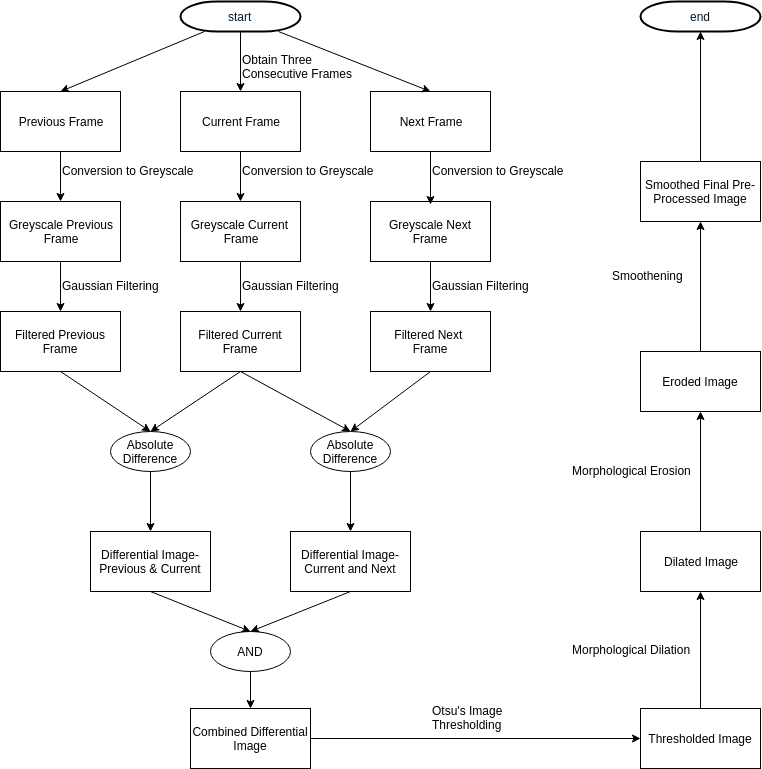
\includegraphics[width=0.7\textwidth]{Foreground_Extraction.png}
\caption{\label{fig:fe}Steps undertaken for extracting the foreground}
\end{figure}
First off, the colored RGB image frames are converted to their Grayscale equivalent to visualize the motion more precisely, followed by filtering of the image frames to reduce noise. The frames are then combined using frame differencing and Boolean operations to a single image which captures the complete motion in an image frame while muting the background. This combined image is thresholded to form a binary image which helps to focus on objects that are of interest. The process is continued by performing certain morphological operations- dilation and erosion that focuses on the shapes in the image by alleviating discontinuity and enhancing the objects in the image. The pre-preocessing stage is concluded by performing a final blurring operation to smoothen the shapes of the objects in the image frame.\par
\newpage


\section{Dataset}


\newpage



\section{Foreground Extraction}
Foreground extraction is the process of separating moving objects in a frame from the static background objects that remain unchanged in every frame. The moving objects are the main focus of tracking algorithms in sports, whether it be tracking a moving player or tracking a high-speed ball or both. Foreground Extraction(or Background Subtraction) is the first step to achieve that goal. \par
As discussed in the literature, there exists two common ways to perform foreground extraction. A difference in consecutive video frames can be taken to identify objects in motion as the value of those pixels will change in the corresponding frame implying motion in those pixels. This is generally performed first by converting the frames to a Grayscale representation and is also followed by Boolean operations to extract the moving parts of the required frame from its previous or next frame.\par
Another method is to first build a background model of the scene in the video, either by recording a video for a small duration of time of a still and empty court or by providing the system with a pre-built background model. By subtracting this background model from a video frame, moving objects can be separated in the frame. Although, the frame-differencing approach is faster, the second approach of creating a background model tends to be more robust towards noise. \par 

\subsection{Conversion to Grayscale}
The frame differencing step is performed after first converting the frames from RGB color space to a Grayscale representation. This is performed using \autoref{eq:grayscale} as defined by the standard set by the International Telecommunication Union, in their recommendation BT.601 (CCIR 601).\par
\begin{equation} \label{eq:grayscale}
    Y = 0.299 R + 0.587 G + 0.114 B
\end{equation}
where, R G \& B represent the color planes of the colors Red, Green and Blue.\par
This conversion is done mainly due to two main reasons. One, the luminance component in an image captures more information as compared to  the chrominance component and is important to distinguish the various visual features in an image. As in human vision, computer vision looks for features in an image based on contrasting patterns in the image pixels as compared to texture and color information. \par 
Second, by converting the image frame to a Grayscale representation, the complexity of further operations gets reduced significantly. A RGB image is composed of three separate 8-bit channels representing the three color planes, but a Grayscale image is an 8 bit image with every pixel a shade of gray with values ranging from 0 to 255. This conversion simplifies the process and reduces computational requirements.\cite{kanan2012color}  \par  
Moreover, as the property of color is not needed to capture the movement, conversion to Grayscale doesn't affect the detection process.  
\subsection{Gaussian Filtering}
Following the conversion to Grayscale representation, the three frames are filtered to remove noise by using a Gaussian filter with a 7x7 kernel size.
A gaussian filter is a weighted average filter with a large weight at the center compared to smaller weights at the boundary of the kernel. The Gaussian filter is formulated as
\begin{equation} \label{eq:Gaussian}
    G(x,y) = \frac{1}{{2\pi \sigma^2}}e^{{{ - \left( {x^2 + y^2 } \right)} \mathord{\left/ {\vphantom {{ - \left( {x - \mu } \right)^2 } {2\sigma ^2 }}} \right. \kern-\nulldelimiterspace} {2\sigma ^2 }}}
\end{equation}
where x and y are the distances of the pixel coordinate from the origin and $\sigma$ is the standard deviation. \par
The standard deviation is represented as inter-pixel space and has an effect on the weight of the elements in the Gaussian kernel. For instance, a large standard deviation corresponds to a greater weight of the boundary elements signifying the  effect of the far-off pixels on the average. This leads to loss of detail in the image along with the noise. A smaller $\sigma$ on the other hand won't have much of an effect as the weights of the pixels off the center will be small. The standard deviation has been calculated using the kernel size with the formula, 
\begin{equation} \label{eq:sigma}
    \sigma = 0.3*((ksize-1)*0.5 - 1) + 0.8
\end{equation}
This means for the kernel-size of 7, the $\sigma$ corresponds to a value of 1.4 pixels.\par
 
The size of the kernel pre-dominantly depends on the size of the objects in the image frames. This means, that the kernel size in a filter varies with every image processing/computer vision application.
A large sized kernel can be in-efficient in removing small salt \& pepper noise whereas a very-small sized kernel might filter out the ball candidate from the frame due to the small size of the squash ball. For this application, a kernel-size of 7x7 strikes the perfect balance to filter out the unnecessary noise in the image frame while maintaining suitable detail in the image to capture the motion.\par

The implementation of the Gaussian Filter used in this project is of that in the Open Source Computer Vision library. The Gaussian filter coefficients are computed using the formula,
\begin{equation}
    G_i= \alpha *e^{-(i-( \texttt{ksize} -1)/2)^2/(2* \texttt{sigma} )^2}
\end{equation}
where, $ i=0..\texttt{ksize}-1$ and $\alpha$ is a scale factor chosen such that $ \sum_i G_i=1.$ 
For a $ksize=7$ and calculating $\sigma$ from \autoref{eq:sigma}, the Gaussian filter coefficients are obtained as \[([0.03125 ],
       [0.109375],
       [0.21875 ],
       [0.28125 ],
       [0.21875 ],
       [0.109375],
       [0.03125 ])\]
It can be observed that these are coefficients for a 1-D filter, to obtain the coefficients for a 2-D Gaussian filter for the same dimensions in x and y directions, the coefficient matrix has to be transposed and multiplied to obtain a 7x7 matrix of Gaussian filter coefficients. This results in the filter coefficient matrix,

\begin{table}[H] \label{tab:coeff}
\resizebox{\textwidth}{!}{%
\begin{tabular}{|l|l|l|l|l|l|l|}
\hline
% C1	&C2	&C3	&C4	&C5	&C6	&C7 \\ \hline
0.0009765625	&0.00341796875	&0.0068359375	&0.0087890625	&0.0068359375	&0.00341796875	&0.0009765625     \\ \hline
0.00341796875	&0.011962890625	&0.02392578125	&0.03076171875	&0.02392578125	&0.011962890625	&0.00341796875 \\ \hline
0.0068359375	&0.02392578125	&0.0478515625	&0.0615234375	&0.0478515625	&0.02392578125	&0.0068359375 \\ \hline
0.0087890625	&0.03076171875	&0.0615234375	&0.0791015625	&0.0615234375	&0.03076171875	&0.0087890625     \\ \hline
	0.0068359375	&0.02392578125	&0.0478515625	&0.0615234375	&0.0478515625	&0.02392578125	&0.0068359375 \\ \hline
	0.00341796875	&0.011962890625	&0.02392578125	&0.03076171875	&0.02392578125	&0.011962890625	&0.00341796875 \\ \hline
	0.0009765625	&0.00341796875	&0.0068359375	&0.0087890625	&0.0068359375	&0.00341796875	&0.0009765625 \\ \hline
\end{tabular}%
}
\caption{7x7 Gaussian Filter Coefficients}
\end{table}

An important property used for optimisation is that of separable convolution. As observed above, the 2D Convolution matrix can be separated into two 1D matrices. Since convolution is associative, instead of performing a convolution of the image with the 2D matrix, two separate convolutions can be performed with the 1D matrices in the horizontal and vertical dimensions i.e. the image can be convolved first with the 1D matrix in the horizontal dimension and then can be convolved with the 1D matrix in the vertical direction. Convolution is much faster with single dimension matrices and the results obtained are same as by a convolution with a 2D matrix. %Equation daale kya?
%https://blogs.mathworks.com/steve/2006/10/04/separable-convolution/


% C1	C2	C3	C4	C5	C6	C7
% 1	0.0009765625	0.00341796875	0.0068359375	0.0087890625	0.0068359375	0.00341796875	0.0009765625
% 2	0.00341796875	0.011962890625	0.02392578125	0.03076171875	0.02392578125	0.011962890625	0.00341796875
% 3	0.0068359375	0.02392578125	0.0478515625	0.0615234375	0.0478515625	0.02392578125	0.0068359375
% 4	0.0087890625	0.03076171875	0.0615234375	0.0791015625	0.0615234375	0.03076171875	0.0087890625
% 5	0.0068359375	0.02392578125	0.0478515625	0.0615234375	0.0478515625	0.02392578125	0.0068359375
% 6	0.00341796875	0.011962890625	0.02392578125	0.03076171875	0.02392578125	0.011962890625	0.00341796875
% 7	0.0009765625	0.00341796875	0.0068359375	0.0087890625	0.0068359375	0.00341796875	0.0009765625


\par
The choice of a Gaussian filter in this application, rather than an averaging filter or a Median filter is motivated by two reasons $-$ performance and efficiency. A Gaussian filter is  a linear filter as compared to the Median filter which is non-linear. This means computation of the new pixel value after convolution with a Gaussian filter is much faster compared to that of a Median Filter.
Another property of the Gaussian filter is that of not preserving any sharp edges in the image. This is especially useful in the scenario of Squash. Squash broadcasts that are used in the project contain a number of Advertisement \& Tournament labelling which if filtered through a Median filter introduces noise due to the sharp edges of those labels. This noise interferes in the Ball Detection stage and makes the detection process more difficult.  

\subsection{Frame Differencing}
The method employed to perform foreground extraction in this Thesis work is that of Frame Differencing. Unlike traditional frame-differencing approaches which takes the difference of two consecutive frames, the approach in this project rather utilizes two frame differencing images generated from three consecutive video frames. The reason for such an approach lies in the fact that the game of Squash has many components that can induce noise. A squash broadcast video with all the advertisement \& score labels, glass fibre walls with reflections and transparent front wall with crowd sitting behind them, generates various noisy components that are difficult to differentiate from the interested motion in the frame. \par 
By utilizing three consecutive frames, i.e. for every frame in which motion has to be separated, two other frames, one preceding frame and one succeeding frame is taken in the process pipeline. Then, two separate frame-difference images are generated by differencing the current frame with the previous one, and by differencing the next frame with the current frame. This process can be observed in figure...... and can be represented in \autoref{eq:currprev} and \autoref{eq:nextcurr}
\begin{equation} \label{eq:currprev}
    \delta_- = I(t) - I(t-1) 
\end{equation} 
\begin{equation} \label{eq:nextcurr}
    \delta_+ = I(t+1) - I(t)
\end{equation}
where, $I(t)$ represent an image frame at time t, and $\delta$ represents a frame differential image.
\par
The process of frame-differencing is quite fast in performance and takes very little time in execution which makes it an optimal approach to isolate motion in a frame.
\par

\subsection{Boolean Combination}
The two frame-differential images are combined together with a Boolean AND operation. This step, ensures the absence of any static objects present throughout those three frames while retaining the motion present in the current frame. Thus, the frame-differential image in \autoref{eq:framediff} contains moving objects present only in the frame that is being analyzed. 
\par

\begin{equation} \label{eq:framediff}
    \delta = \delta_- \wedge \delta_+
\end{equation}
\newpage

\section{Thresholding}
The frame-differential image is processed further and converted into a binary image by performing a thresholding operation. The conversion from a grayscale image to a binary image is a common step performed in image processing and computer vision applications to detect regions of interest. By converting into a binary image, the processing is simplified as there are either pixels of value '1' which are of interest or of value '0' which are not of any interest in a video frame. \par
There are various thresholding methods commonly utilized in computer vision applications that involve either the user providing the threshold value such as the Simple Thresholding method, or there are methods that derive the optimum threshold value such as the Adaptive Threshold method. The simple thresholding method works for the cases where  the knowledge of a global threshold value is known before-hand. The adaptive threshold method is more applicable to cases where the threshold value is expected to change quite frequently and is never constant such as in images with a lot of varying information (per frame) in it. \par 
There is another popular image threshold method, Otsu's Binarization, which has been utilized in this project. Otsu's thresholding method works well for a bimodal image, where there are two peaks of pixel values in the histogram of the image. This means, for images that have a very clear separation between the foreground and the background, the Otsu's method works well. Otsu's thresholding method automatically calculates the optimum threshold value to divide the group of pixels in the image. The way it does that is by finding a threshold value which lies in between the two peaks in the histogram of the image, which minimizes the variance to both groups of pixels being thresholded. It is easy to observe why this method is the ideal choice to perform the thresholding operation, as in each frame there is always a majority of pixels with the value near to '0' that correspond as the background in the frame, and a very few pixels with larger values(grayish-white pixels) that indicate objects with motion in the frame. By separating these two types of pixels, the resulting thresholded image quite clearly shows the moving objects in the frame over a black background. \par
%histogram image 
\newpage


\section{Morphological Operations}
The frame difference and thresholding operations result in a binary representation of the video frame which is highly disconnected and infused with noise. This implies the need to perform further image processing operations to further refine the image and remove the noise from the binary image.\par

For this task, morphological operations are performed to improve the 
\newpage
\section{Final Touch}
The choice of a median filter is made in accordance with the fact that the median filter uses an existing pixel value from the surrounding pixels as the new pixel value. This is different as compared with an Average filter or a Gaussian filter which can completely change the pixel value to one that doesn't exist in the frame. By using an existing pixel value, there is no loss of information from the frame especially considering the fact that the size of the ball in the frame is too small, while it simultaneously filters out small noise present in the frame, making a median filter as the ideal choice.\par
\newpage
\newpage
\bibliographystyle{ieeetr}
\bibliography{bibliography.bib}
\end{document}